\documentclass[11pt]{article}

% --- Page + fonts (Palatino: clean, journal-standard look) ---
\usepackage[utf8]{inputenc}
\usepackage[T1]{fontenc}
\usepackage[margin=1.1in]{geometry}
\usepackage{mathpazo}
\usepackage{amsmath, amssymb, amsthm}
\usepackage{graphicx}
\usepackage{booktabs}
\usepackage{caption}
\usepackage{microtype}
\usepackage{setspace}
\usepackage{enumitem}
\usepackage[authoryear,round]{natbib}
\usepackage{titlesec}
\usepackage{titling}
\usepackage{fancyhdr}
\usepackage[most]{tcolorbox}
\usepackage{hyperref}
\hypersetup{colorlinks=true, linkcolor=black, citecolor=black, urlcolor=blue}

\linespread{1.05}
\setlength{\parskip}{0.55em}
\setlength{\parindent}{0pt}

% --- Caption styling ---
\captionsetup[table]{labelfont=bf, font=small, skip=4pt}
\captionsetup[figure]{labelfont=bf, font=small, skip=4pt}

% --- Section heading style (refined, journal-like) ---
\titleformat{\section}{\large\bfseries\scshape}{\thesection}{0.6em}{}
\titleformat{\subsection}{\normalsize\bfseries}{\thesubsection}{0.6em}{}
\titlespacing*{\section}{0pt}{1.3em}{0.5em}
\titlespacing*{\subsection}{0pt}{0.9em}{0.3em}

% --- Running header ---
\pagestyle{fancy}
\fancyhf{}
\renewcommand{\headrulewidth}{0.4pt}
\fancyhead[L]{\small\scshape Racial Incidence of Monetary Contractions}
\fancyhead[R]{\small\thepage}
\fancypagestyle{plain}{\fancyhf{}\fancyhead[R]{\small\thepage}\renewcommand{\headrulewidth}{0pt}}

% --- Graphics path ---
\graphicspath{{figures/}}

% --- Plain-language summary box ---
\newtcolorbox{summarybox}{
  colback=gray!5, colframe=gray!55, boxrule=0.5pt, arc=2pt,
  left=10pt, right=10pt, top=8pt, bottom=8pt,
  fonttitle=\bfseries, title=Plain-Language Summary}

% --- Title block ---
\title{\bfseries Between Metros, Not Within:\\[2pt]
\large The Racial Incidence of Identified Monetary\\ Contractions on Local Employment}
\author{Abdallah Dalis\thanks{DePaul University. Email: \texttt{dalisabdallah@gmail.com}.
Replication code and data: \texttt{Dalis\_Abdallah\_Part3\_Code.R}. This is the third
installment of a research program on the local labor-market transmission of monetary
policy. I thank Prof.\ Jin Man Lee for advising the program. All errors are my own.}}
\date{Working paper \textperiodcentered\ \today}

\begin{document}
\maketitle
\thispagestyle{plain}

% =============================================================================
% STATUS: complete. All sections drafted from verified results; numbers match
% Dalis_Abdallah_Part3_Code.R (Mac-verified to 4 decimals). Literature review
% included. All 11 citations verified against publisher records (June 2026).
% =============================================================================

\begin{abstract}
\noindent Monetary contractions reduce employment, but whether the cost falls
disproportionately on communities of color is contested and rarely estimated with clean
identification. Using Jorda local projections across 2{,}884 U.S.\ counties from 2002 to
2019, I interact identified Bauer--Swanson monetary policy surprises with predetermined
2000 Census racial composition. Counties with higher Black population shares experience
larger employment contractions after an identified tightening; the gradient is robust to
controls for county size, income, and industry exposure, and income strengthens rather
than attenuates it. The estimate is directionally stable but imprecise, as expected from a
short high-frequency surprise series. A within-metropolitan decomposition is decisive:
replacing national time effects with metropolitan-by-quarter effects reverses the sign.
The gradient is a between-metropolitan phenomenon. Higher-Black metros contract more as
whole labor markets, while within a metro, higher-Black counties do not. The racial
incidence of monetary contractions operates across metropolitan areas, not within them,
pointing to regional and industrial structure rather than a within-market race effect.

\vspace{0.6em}
\noindent\textbf{Keywords:} monetary policy transmission; local labor markets; racial
inequality; local projections; high-frequency identification.

\noindent\textbf{JEL:} E52, J15, R23, E24.
\end{abstract}

\begin{summarybox}
When the Federal Reserve raises interest rates to slow the economy, some people lose their
jobs. This paper asks a simple question: do places with more Black residents lose more of
those jobs? To answer it credibly, I use only the \emph{surprise} part of Fed decisions,
the piece markets did not see coming, so that I am measuring the effect of policy rather
than a coincidence.

Three things emerge. First, counties with larger Black populations do tend to lose more
jobs after a surprise rate increase. The direction matches the concern, though the data is
noisy enough that the result is not statistically airtight. Second, this is not simply a
story about poorer, smaller, or differently-industried places: the pattern holds when those
factors are held constant, and accounting for income actually makes it sharper.

Third, and most important, the disadvantage shows up \emph{between cities}, not between
neighbors. Heavily-Black metropolitan areas, taken as whole labor markets, contract more
than other metros. But inside a single metro, a county with a larger Black share is not hit
harder than a whiter county next door. So the cost is tied to which metropolitan economy a
community belongs to, with its particular industries and regional exposure, rather than to
race operating block by block.

The honest limit is precision. With about eighteen years of these surprises, the pattern is
clear in direction and survives every reasonable objection, but it cannot be pinned to an
exact number. The contribution is a clean, well-identified design and a robust structural
finding about \emph{where} the disadvantage lives.
\end{summarybox}

% =============================================================================
\section{Introduction}
% =============================================================================
Monetary policy is not distributionally neutral. A growing literature documents that Black
employment is markedly more cyclically sensitive than white employment
\citep{CajnerEtAl2017}, and that episodes of monetary tightening widen racial gaps in labor
market outcomes \citep{CarpenterRodgers2004, SeguinoHeintz2012}. A parallel literature shows
that the transmission of policy is geographically uneven, varying with regional industrial
composition \citep{CarlinoDeFina1998}. Together these strands raise a natural question about
\emph{incidence}: when contractionary policy destroys jobs, who bears the loss?

Two obstacles have kept the question hard to answer cleanly. First, distributional estimates
typically use the realized federal funds rate or other aggregate series, which over the
2002--2019 window are contaminated by endogeneity and by the information effect, the tendency
of announced policy to bundle the central bank's private read on the economy. The earlier
installments of this program show that, in this window, the endogenous funds rate even
delivers a perverse positive employment response that the identified surprise corrects.
Second, a county-level racial gradient can reflect race or any of the things race is
correlated with: county size, income, industry mix, and region. Distinguishing these
requires both an identified shock and a research design that isolates the comparison.

This paper supplies both. I hold fixed the identified design of Part~2, a Jorda local
projection driven by the Bauer--Swanson high-frequency monetary policy surprise
\citep{BauerSwanson2023, Jorda2005}, and swap the heterogeneity dimension from industry
exposure to predetermined 2000 Census racial composition. I then build a control ladder
(size, income, industry exposure) and, decisively, a within-metropolitan comparison that
holds the metro-quarter fixed.

Three findings follow. (i)~The surprise-by-Black-share gradient is negative and deepens with
the horizon, consistent with disproportionate incidence, but is imprecise. (ii)~It survives
the control ladder; income sharpens rather than absorbs it. (iii)~It is a between-metropolitan
phenomenon: within-metro identification reverses the sign. The disadvantage is attached to
which metropolitan economy a community sits in, not to its racial composition relative to
neighbors. The remainder of the paper presents the data (Section~2), the estimator and
identification (Section~3), the results figure by figure (Section~4), and a discussion of
mechanisms, caveats, and what the between-metro location of the effect implies (Sections 5--6).

% =============================================================================
\section{Literature Review}
% =============================================================================
This paper sits at the intersection of three literatures: the high-frequency
identification of monetary policy shocks, the regional and local transmission of those
shocks, and their distributional incidence across racial groups.

\subsection{Identifying monetary policy shocks}
A core difficulty in measuring the effects of monetary policy is that the policy rate
responds to the economy, so realized rate changes confound policy with the conditions that
provoked it. \citet{Jorda2005} introduced local projections as a flexible alternative to
vector autoregressions for tracing dynamic responses, estimating a separate regression at
each horizon and avoiding the recursive extrapolation that makes VAR impulse responses
fragile; this is the estimator I adopt. High-frequency identification narrows the
remaining endogeneity by measuring the surprise component of policy in a tight window
around announcements, but \citet{NakamuraSteinsson2018} show that these surprises are
themselves contaminated by an information effect: a tightening surprise can raise private
output forecasts, as if the announcement reveals the central bank's favorable read on the
economy, biasing estimated effects toward zero or the wrong sign. \citet{BauerSwanson2023}
offer an alternative explanation, arguing the apparent information effect reflects the
central bank and the public responding to the same publicly available news, and construct
an orthogonalized surprise series that purges this predictable component. I use their
orthogonalized surprise as the identified shock, which is what allowed Part~2 of this
program to overturn the perverse positive employment response that the endogenous funds
rate produces over the 2002--2019 window.

\subsection{Regional and local transmission}
Monetary policy does not land evenly across places. \citet{CarlinoDeFina1998} document
that the employment response to policy varies systematically across U.S.\ regions, with
the differences traceable to regional variation in industry mix and the interest
sensitivity of local production. This motivates a place-based design but also warns that
any cross-sectional gradient may reflect industrial composition rather than the
characteristic of interest. The natural design for such gradients is the shift-share or
Bartik approach \citep{Bartik1991}, in which a local exposure share is interacted with an
aggregate shock; \citet{GPSS2020} clarify that identification in these designs rests on the
exogeneity of the predetermined shares. Parts~1 and~2 of this program applied exactly this
logic with industry-exposure shares and found that the exposure gradient did not survive
controlling for county size. Part~3 keeps the identified-shock-times-predetermined-share
structure but replaces industry exposure with racial composition.

\subsection{Distributional incidence by race}
A distinct literature asks who bears the employment cost of contractions.
\citet{CarpenterRodgers2004}, using recursive VARs and distributed-lag models on aggregate
series, find that the employment of minorities, and of African Americans in particular, is
more sensitive to contractionary policy than that of whites, operating mainly through
higher unemployment rather than reduced participation. \citet{SeguinoHeintz2012}, using
U.S.\ state-level panel data from 1979 to 2008, find that the unemployment cost of monetary
tightening falls most heavily on Black women and Black men, that the effect is not
race-neutral, and, most relevant here, that the relative cost borne by subordinate groups
\emph{varies with the Black share of the population}. \citet{CajnerEtAl2017} provide the
background regularity: Black unemployment is both higher and substantially more cyclical
than white unemployment, driven largely by a higher risk of job loss, while the
Hispanic-white gap is smaller and mostly explained by educational composition, a pattern
that anticipates the null Hispanic gradient I find.

\subsection{The gap this paper fills}
Prior distributional work is built almost entirely on national time-series or state-level
panels, and on the realized policy rate or unidentified surprises. Two gaps follow. First,
the distributional question has not been asked with a cleanly identified shock at a fine
geographic scale, leaving open whether the documented racial gradient reflects policy or
the endogeneity and information-effect problems that Part~2 shows are first-order in this
window. Second, and more fundamentally, the existing place-based estimates do not separate
\emph{between}-metropolitan from \emph{within}-metropolitan variation. \citet{SeguinoHeintz2012}
show the cost varies with the Black population share, but a state-level design cannot tell
whether that gradient operates across metropolitan labor markets or between adjacent
counties inside one. This paper supplies both: an identified surprise interacted with
predetermined county racial composition, a control ladder that nets out size, income, and
industry exposure, and a within-metro comparison that locates where the gradient actually
lives.

% =============================================================================
\section{Data}
% =============================================================================
The estimation sample is a panel of 2{,}884 U.S.\ counties observed quarterly from 2002Q1
through 2019Q4 (72 quarters), inherited intact from Part~2.

\textbf{Employment.} County employment is the QCEW quarterly establishment count
(\texttt{month3\_emplvl}); the outcome at horizon $h$ is the log-employment change
$100\,(\ell_{i,t+h}-\ell_{i,t-1})$.

\textbf{Identified monetary shock.} The Bauer--Swanson orthogonalized high-frequency
monetary policy surprise \citep{BauerSwanson2023}, summed to quarterly frequency. The
orthogonalization purges the surprise of the predictable macro-news component that drives
the Fed information effect.

\textbf{Predetermined heterogeneity dimensions.} County racial composition is the
predetermined 2000 Census share Black-alone and Hispanic (April~1, 2000 population base),
so the shares cannot respond to anything in the 2002--2019 sample. Predetermined controls:
log 2000 population (size); log 2000 median household income (Census~2000 SF3, table
P053001); and the Part~1--2 industry-exposure share (2002 CBP construction-plus-manufacturing
employment share). All dimensions are standardized, so coefficients are read per
one-standard-deviation of the share.

\textbf{Metropolitan grouping.} Counties are mapped to Core-Based Statistical Areas via the
Census 2020 delineation. The within-metro analysis retains counties in a CBSA with at least
two sample counties (1{,}110 counties across 300 CBSAs), since metro-by-quarter effects
require within-metro variation.

% =============================================================================
\section{Methodology}
% =============================================================================
The estimator is a Jorda local projection \citep{Jorda2005}. For each horizon
$h = 0,\dots,12$ quarters,
\begin{equation}
100\,(\ell_{i,t+h}-\ell_{i,t-1}) \;=\; \alpha_i^h + \delta_t^h
   \;+\; \theta_h \,\bigl(s_t \times d_i\bigr) \;+\; \mathbf{x}_{i}'\boldsymbol{\gamma}_h \;+\; \varepsilon_{i,t+h},
\label{eq:lp}
\end{equation}
where $s_t$ is the identified surprise, $d_i$ a standardized predetermined county
characteristic (Black share in the headline specification), $\alpha_i^h$ county fixed
effects, and $\delta_t^h$ time fixed effects. Because $s_t$ is national, the time effects
absorb its main effect; $\theta_h$ is identified from the interaction of the shock with
cross-county differences in $d_i$. A negative $\theta_h$ means higher-share counties contract
more after an identified tightening.

\textbf{Control ladder.} I add $s_t\times\log\text{pop}_i$, $s_t\times\log\text{inc}_i$, and
$s_t\times\text{exposure}_i$ sequentially, so the racial gradient is read net of the
county-size confound that absorbed the Part~2 industry gradient, of income, and of the
industry channel.

\textbf{Within-metro identification.} The key decomposition replaces the national time effect
$\delta_t^h$ with a metro-by-quarter effect $\delta_{c(i),t}^h$, comparing higher- and
lower-Black counties \emph{inside the same metro-quarter}. County and metro-by-quarter effects
are non-nested and absorbed by \texttt{fixest::feols}.

\textbf{Inference.} Standard errors are clustered by quarter in the baseline. As a robustness
check I report Driscoll--Kraay standard errors \citep{DriscollKraay1998}, which additionally
allow serial correlation across quarters. The surprise series spans 72 quarters, so estimates
are expected to be imprecise; I report this rather than select favorable horizons.

\textbf{Reproducibility.} All results are produced by \texttt{Dalis\_Abdallah\_Part3\_Code.R}
(Sections 1--7) and were verified on the author's machine.

% =============================================================================
\section{Results}
% =============================================================================

\subsection{The baseline gradient and a validation check}
Figure~\ref{fig:incidence} plots $\theta_h$ for the surprise interacted with Black share,
Hispanic share, and (as a validation against Part~2) industry exposure. The exposure line
reproduces Part~2: negative and monotonically deepening to $-2.39$ by $h{=}12$, confirming the
pipeline. The Black-share gradient is negative at ten of thirteen horizons, deepening to
roughly $-1.06$ by $h{=}12$, but statistically insignificant throughout ($|t| < 0.9$).
Hispanic share is a null at every horizon. The direction is consistent with disproportionate
incidence; the precision is not.

\begin{figure}[tbp]
\centering
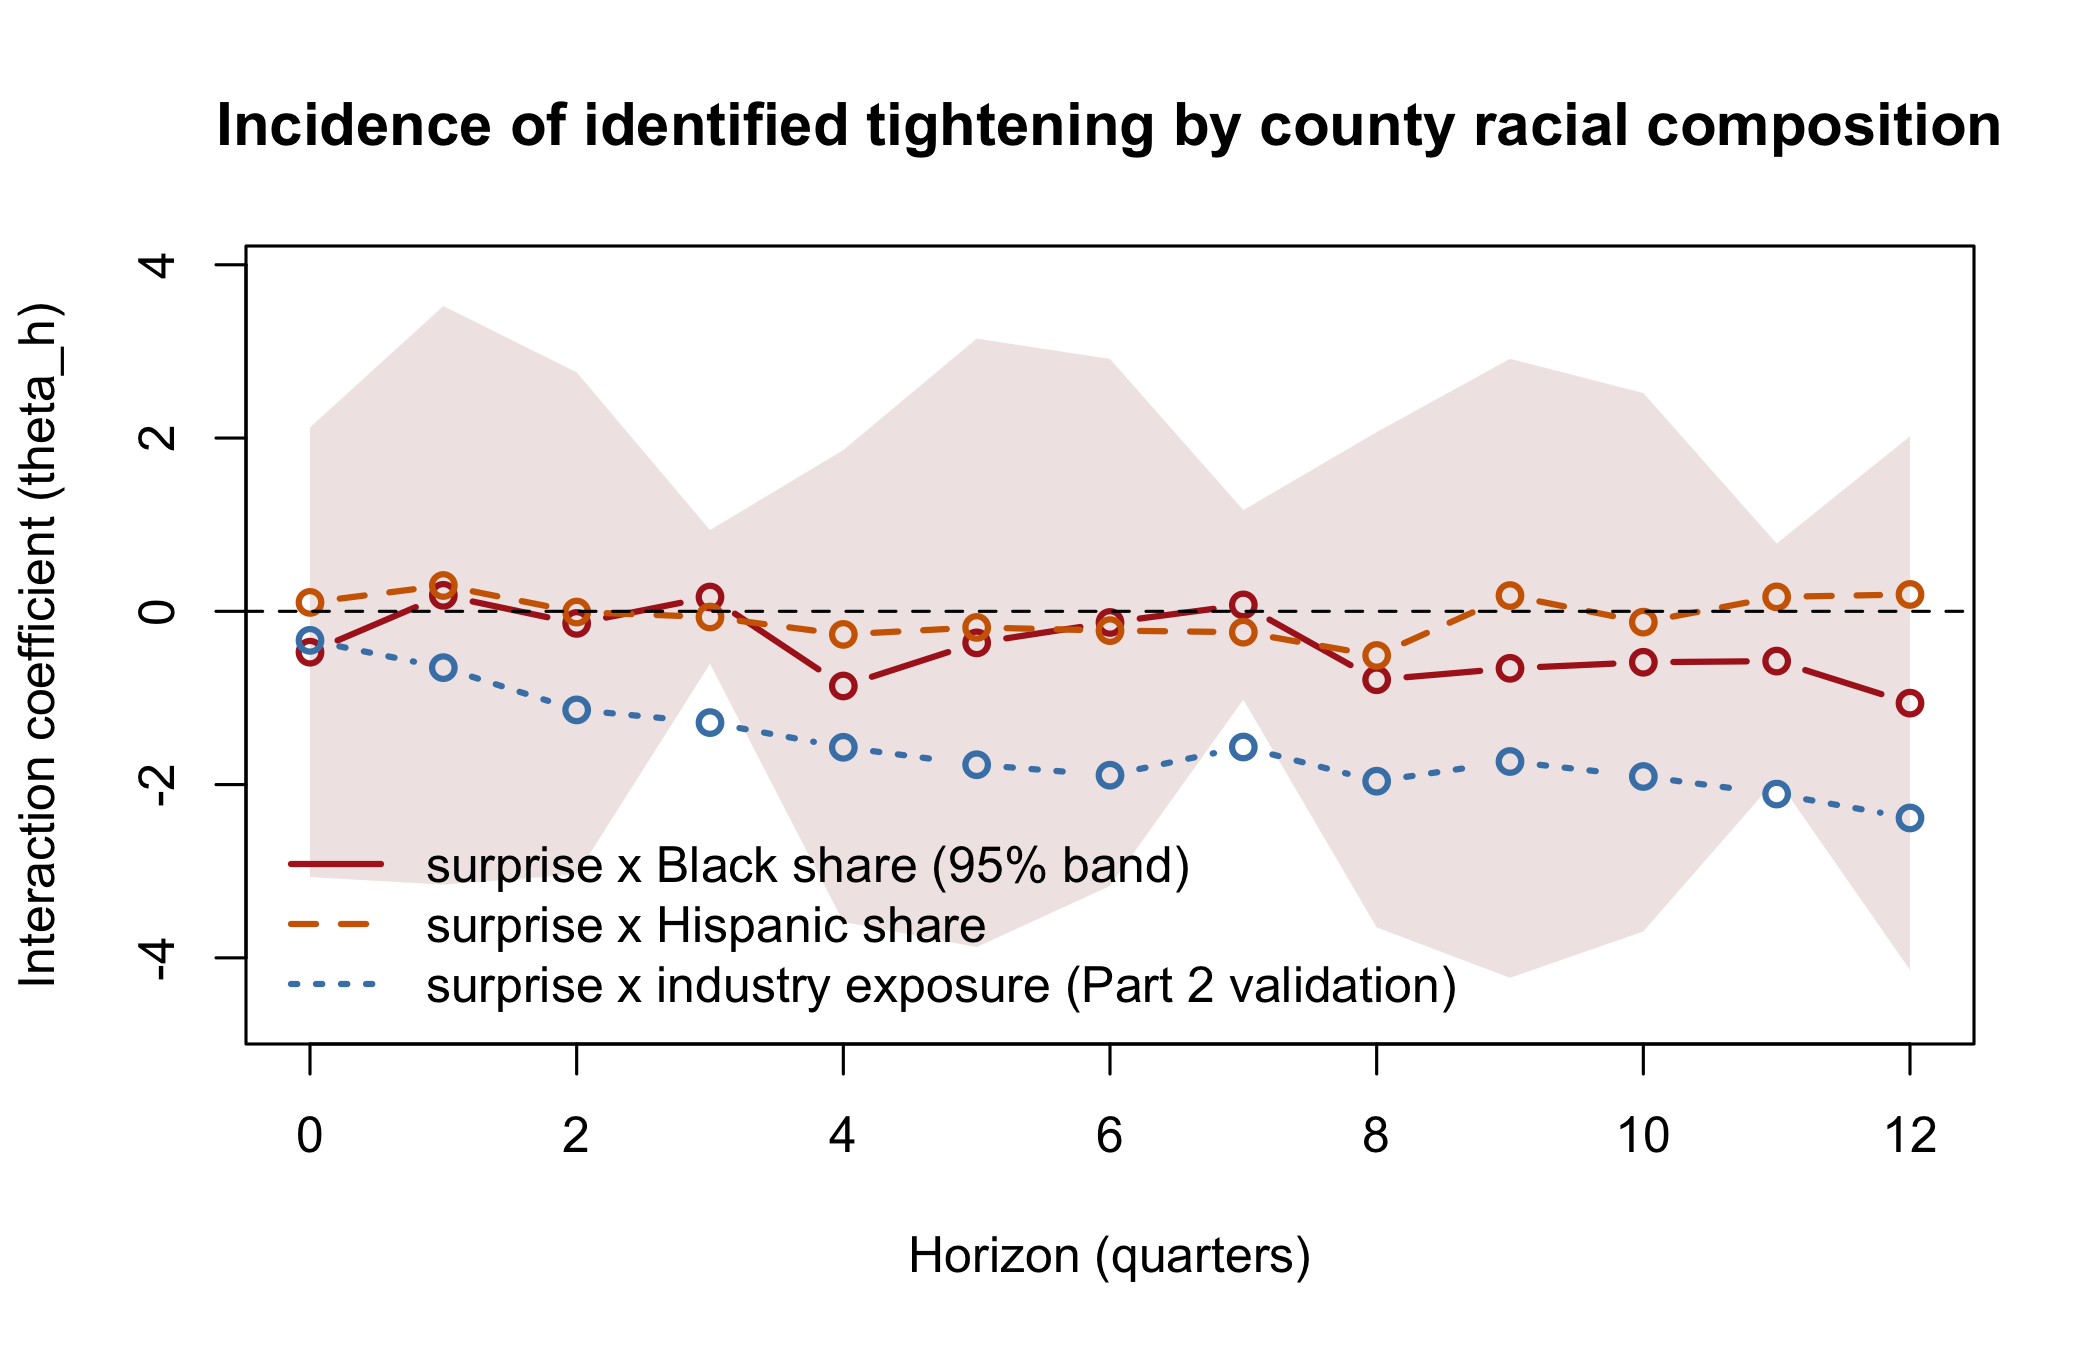
\includegraphics[width=0.78\linewidth]{fig_part3_incidence.png}
\caption{Interaction coefficient $\theta_h$ from Eq.~\eqref{eq:lp}: identified surprise
$\times$ standardized Black share (with 95\% band), Hispanic share, and industry exposure
(Part~2 validation). County and quarter fixed effects; quarter-clustered SE.}
\label{fig:incidence}
\end{figure}

\subsection{The control ladder: income sharpens, not absorbs}
Table~\ref{tab:ladder} and Figure~\ref{fig:ladder} report the Black coefficient as controls
are added. The gradient survives netting out county size, the confound that eliminated the
Part~2 industry gradient. Adding 2000 median household income does not absorb it; it
\emph{sharpens} it at the long horizons (from $-1.06$ to $-1.19$ at $h{=}12$, with $|t|$
approaching $1.0$ at $h{=}11$), because poorer and higher-Black counties partly offset, so
holding income fixed widens the racial gap. Adding industry exposure leaves it essentially
unchanged. The gradient is therefore not size, income, or industry mix in disguise; it remains
imprecise.

\begin{table}[tbp]
\centering
\caption{Black-share coefficient $\theta_h$ across the control ladder (national time FE, full
sample $n=2{,}884$ counties). Selected horizons; $t$-statistics in parentheses,
quarter-clustered.}
\label{tab:ladder}
\begin{tabular}{lcccc}
\toprule
Horizon & Black alone & $+\log$pop & $+\log$pop$+$inc & $+\log$pop$+$inc$+$exp \\
\midrule
$h{=}0$  & $-0.47\;(-0.36)$ & $-0.46\;(-0.40)$ & $-0.46\;(-0.56)$ & $-0.46\;(-0.56)$ \\
$h{=}4$  & $-0.86\;(-0.62)$ & $-0.66\;(-0.55)$ & $-0.70\;(-0.73)$ & $-0.70\;(-0.72)$ \\
$h{=}8$  & $-0.79\;(-0.54)$ & $-0.54\;(-0.43)$ & $-0.75\;(-0.69)$ & $-0.75\;(-0.68)$ \\
$h{=}11$ & $-0.57\;(-0.83)$ & $-0.38\;(-0.79)$ & $-0.93\;(-1.02)$ & $-0.92\;(-1.03)$ \\
$h{=}12$ & $-1.06\;(-0.67)$ & $-0.77\;(-0.58)$ & $-1.19\;(-0.90)$ & $-1.18\;(-0.90)$ \\
\bottomrule
\end{tabular}
\end{table}

\begin{figure}[tbp]
\centering
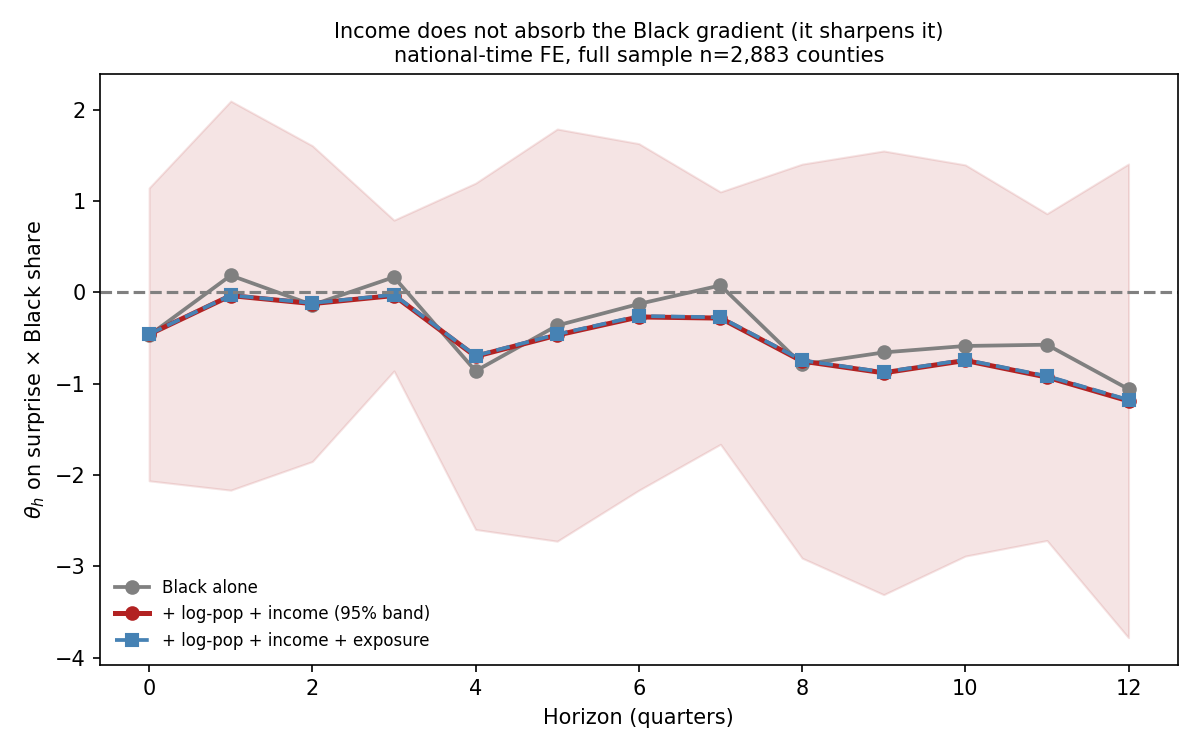
\includegraphics[width=0.78\linewidth]{fig_part3_income_ladder.png}
\caption{The Black-share gradient under successive controls. Income does not absorb the
gradient; it sharpens it at long horizons. National time FE, full sample.}
\label{fig:ladder}
\end{figure}

\subsection{Between metros, not within}
Figure~\ref{fig:withinbetween} and Table~\ref{tab:withinbetween} report the decomposition that
reframes the paper. On the identical metro-county sample, replacing the national time effect
with a metro-by-quarter effect flips the sign of the Black gradient from negative to positive
(at $h{=}12$, from $-0.36$ between-and-within to $+0.89$ within-metro). Because only the
fixed-effect structure changes, this is not a sample artifact. The negative gradient lives in
the \emph{between-metropolitan} variation: metros with higher Black population shares contract
more after identified tightening. Inside a given metro, higher-Black counties do not. All
estimates remain imprecise.

\begin{figure}[tbp]
\centering
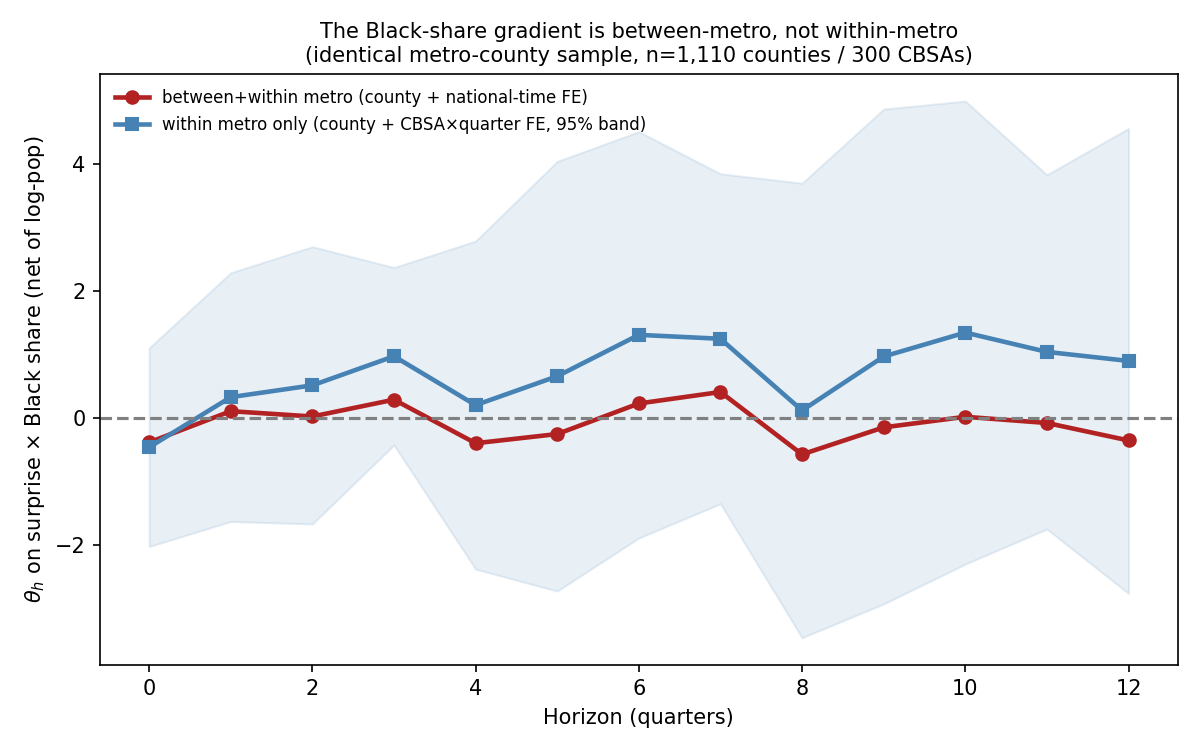
\includegraphics[width=0.78\linewidth]{fig_part3_within_vs_between.png}
\caption{Black-share gradient, identical metro-county sample ($n=1{,}110$ counties, 300
CBSAs): between-plus-within (county $+$ national-time FE) vs within-metro
(county $+$ metro$\times$quarter FE, 95\% band).}
\label{fig:withinbetween}
\end{figure}

\begin{table}[tbp]
\centering
\caption{Between- vs within-metro Black-share coefficient $\theta_h$ (metro sample, net of log
population). Selected horizons; quarter-clustered SE in parentheses.}
\label{tab:withinbetween}
\begin{tabular}{lcc}
\toprule
Horizon & Between $+$ within (national-time FE) & Within metro (metro$\times$quarter FE) \\
\midrule
$h{=}0$  & $-0.39\;(1.02)$ & $-0.46\;(0.80)$ \\
$h{=}4$  & $-0.40\;(1.13)$ & $\phantom{-}0.20\;(1.32)$ \\
$h{=}8$  & $-0.58\;(1.14)$ & $\phantom{-}0.11\;(1.83)$ \\
$h{=}12$ & $-0.36\;(1.17)$ & $\phantom{-}0.89\;(1.87)$ \\
\bottomrule
\end{tabular}
\end{table}

\subsection{Robustness}
Two checks complete the picture. First, entering Black and Hispanic shares jointly leaves the
Black gradient essentially unchanged ($-1.17$ at $h{=}12$) while Hispanic remains null, so the
gradient is not Hispanic composition in disguise. Second, Driscoll--Kraay standard errors do
not weaken the result; at the long horizons they are if anything tighter than the clustered
errors ($|t|\approx 1.5$ at $h{=}11$). The imprecision is a property of the 72-quarter surprise
series, not of the inference method or the controls.

% =============================================================================
\section{Discussion}
% =============================================================================
\textbf{Review.} The headline is a direction that is robust and a magnitude that survives
controls, paired with precision that never crosses conventional thresholds, and a
decomposition that locates the entire negative gradient between metropolitan areas rather than
within them.

\textbf{Interpretation.} A between-metro racial gradient that does not survive within-metro
comparison points away from a within-labor-market race mechanism and toward the characteristics
that distinguish higher-Black metros: industrial composition, regional exposure, and local
policy regimes. This rhymes with the program's arc. Part~2 was ``identification, not
aggregation''; Part~3 is ``between, not within.'' It is consistent with a literature in which
Black employment is more cyclically exposed \citep{CajnerEtAl2017} and tightening widens racial
gaps \citep{CarpenterRodgers2004, SeguinoHeintz2012}, while clarifying that, in this sample,
the place-based version of that exposure is a cross-metro phenomenon.

\textbf{Caveats and risks.}
\begin{itemize}[nosep]
  \item \textbf{Power.} Seventy-two quarters of an identified surprise leave every estimate
        imprecise. The contribution is a clean, well-identified design and a robust
        \emph{pattern}, not a precise point estimate.
  \item \textbf{Place vs people.} County composition proxies who bears the cost; place-level
        incidence is not worker-level incidence.
  \item \textbf{Information effect.} Residual Nakamura--Steinsson information-effect
        contamination of the surprise series \citep{NakamuraSteinsson2018} carries over from
        Part~2 and is the deepest unresolved threat; it is discussed, not claimed solved.
\end{itemize}

% =============================================================================
\section{Conclusion}
% =============================================================================
Identified monetary contractions fall harder on metropolitan areas with larger Black
populations, taken as whole labor markets, but not on higher-Black counties relative to whiter
counties within the same metro. The estimate is directionally robust, survives controls for
size, income, and industry as well as joint entry of Hispanic share and a more demanding
standard-error treatment, and is honestly underpowered given the length of the surprise series.

Two implications follow. For research, distributional analysis of monetary policy should
condition on the metropolitan scale, since aggregating or pooling across metros can attribute
to race what is really cross-metro structure, while a naive within-metro look can miss the
disadvantage entirely. For policy, the lever that matters is the differential exposure of
metropolitan economies, their industries and regions, rather than a county-level racial channel.
The most promising next steps are a longer or extended surprise series to lift power,
worker-level outcomes to move from place-based to person-based incidence, and a decomposition of
the between-metro gradient into its industrial and regional components.

% =============================================================================
\section*{Acknowledgements}
% =============================================================================
Data: U.S.\ Bureau of Labor Statistics (QCEW), U.S.\ Census Bureau (2000 Census, County
Business Patterns, CBSA delineation), Federal Reserve Economic Data, and the Bauer--Swanson
monetary policy surprise series (Federal Reserve Bank of San Francisco). Program advisor:
Prof.\ Jin Man Lee, DePaul University.

% =============================================================================
% REFERENCES --- all 11 entries verified against publisher records (June 2026).
% =============================================================================
\begin{thebibliography}{99}
\setlength{\itemsep}{2pt}

\bibitem[Bartik(1991)]{Bartik1991}
Bartik, T.~J. (1991). \textit{Who Benefits from State and Local Economic Development Policies?}
W.E.\ Upjohn Institute.

\bibitem[Bauer and Swanson(2023)]{BauerSwanson2023}
Bauer, M.~D., and Swanson, E.~T. (2023). An Alternative Explanation for the ``Fed Information
Effect.'' \textit{American Economic Review}, 113(3), 664--700.

\bibitem[Cajner et al.(2017)]{CajnerEtAl2017}
Cajner, T., Radler, T., Ratner, D., and Vidangos, I. (2017). Racial Gaps in Labor Market
Outcomes in the Last Four Decades and over the Business Cycle. \textit{Finance and Economics
Discussion Series} 2017-071, Federal Reserve Board.

\bibitem[Carlino and DeFina(1998)]{CarlinoDeFina1998}
Carlino, G., and DeFina, R. (1998). The Differential Regional Effects of Monetary Policy.
\textit{Review of Economics and Statistics}, 80(4), 572--587.

\bibitem[Carpenter and Rodgers(2004)]{CarpenterRodgers2004}
Carpenter, S.~B., and Rodgers, W.~M. (2004). The Disparate Labor Market Impacts of Monetary
Policy. \textit{Journal of Policy Analysis and Management}, 23(4), 813--830.

\bibitem[Driscoll and Kraay(1998)]{DriscollKraay1998}
Driscoll, J.~C., and Kraay, A.~C. (1998). Consistent Covariance Matrix Estimation with
Spatially Dependent Panel Data. \textit{Review of Economics and Statistics}, 80(4), 549--560.

\bibitem[Goldsmith-Pinkham et al.(2020)]{GPSS2020}
Goldsmith-Pinkham, P., Sorkin, I., and Swift, H. (2020). Bartik Instruments: What, When, Why,
and How. \textit{American Economic Review}, 110(8), 2586--2624.

\bibitem[Jorda(2005)]{Jorda2005}
Jorda, O. (2005). Estimation and Inference of Impulse Responses by Local Projections.
\textit{American Economic Review}, 95(1), 161--182.

\bibitem[Nakamura and Steinsson(2018)]{NakamuraSteinsson2018}
Nakamura, E., and Steinsson, J. (2018). High-Frequency Identification of Monetary
Non-Neutrality: The Information Effect. \textit{Quarterly Journal of Economics}, 133(3),
1283--1330.

\bibitem[Seguino and Heintz(2012)]{SeguinoHeintz2012}
Seguino, S., and Heintz, J. (2012). Monetary Tightening and the Dynamics of US Race and Gender
Stratification. \textit{American Journal of Economics and Sociology}, 71(3), 603--638.

\end{thebibliography}

\end{document}
